\section{Introduction}
Dark matter (DM) halos are the basic building blocks of the cosmos. DM particles within halos are collisionless, conserving their orbital energy, and are supported through dispersion \cite{Wetzel2015}. In contrast, gas loses its orbital energy, gathering and clumping in the center of halos, triggering star and eventually galaxy formation \cite{Frenk2012}. Understanding DM halos is crucial for testing and improving lambda cold dark matter ($\Lambda$CDM) theory, the leading paradigm for cosmic structure and evolution. 

$\Lambda$CDM inhabits the framework of general relativity and adopts a particle nature for dark matter to describe the cosmos \cite{Bullock2017}. $\Lambda$CDM has been largely successful in describing the history, structure, and evolution cosmos, but can be improved by further investigating the nature of DM halos. Given their significance in the assembly of DM halos, \textit{galaxy mergers} offer a unique perspective to peer into the nature of galaxy evolution and test $\Lambda$CDM cosmology.

Within $\Lambda$CDM theory, the Navarro-Frenk-White (NFW) density profile \cite{Navarro1997}, Einsasto profile \cite{Navarroetal2004}, and Hernquist profile \cite{Hernquist1990} are commonly used to describe DM halos. These profiles are supported by $\Lambda$CDM theory and were formulated with the aid of N-body simulations. N-body simulations have been widely used to uncover the nature of DM halos. For example, \cite{Frenk2012} used a number of simulations, such as the Aquarius simulation seen in \textbf{Figure \ref{Aquarius halo}}, to determine that the mass in halos is concentrated toward the center, aspherical, and contains substructures especially in the outermost regions. It was also found from \cite{Davis1985} and the friends-of-friends algorithm that CDM halos are often triaxial and rotate slowly.

\begin{wrapfigure}[24]{hr}{0.5\textwidth}
  \begin{center}
    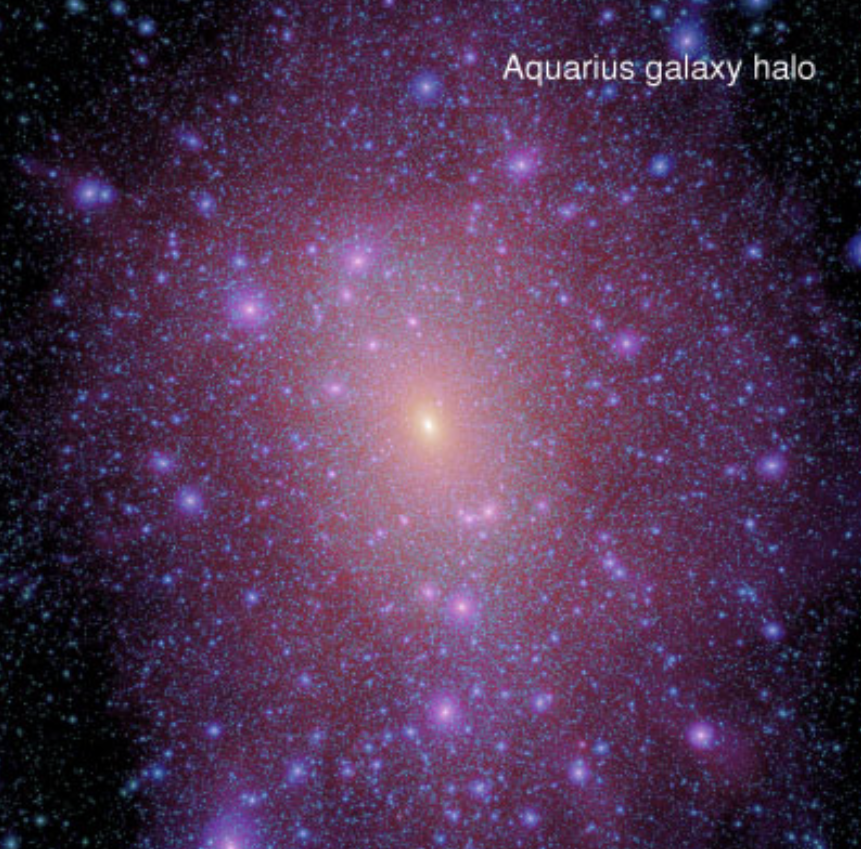
\includegraphics[width=0.48\textwidth]{Figures/Aquariushalo.png}
  \end{center}
  \caption{Simulated dark matter halo from \cite{Frenk2012}. Aquarius galaxy has similar mass to the Milky Way.}
  \label{Aquarius halo}
\end{wrapfigure}

Observations have challenged $\Lambda$CDM theory on smaller scales. The cusp-core problem (first proposed by \cite{Flores1994}) is the most testable challenge of $\Lambda$CDM when analyzing dark matter halos. $\Lambda$CDM theory suggests that the velocity profile of dark matter halos rises steeply at small radii akin to $\rho(r) \propto r^{-\gamma}$ where $\gamma$ is dependent on the mass of the galaxy \cite{Bullock2017}. Instead, some velocity profiles, especially from DM-dominant galaxies, are observed to exhibit flatter slopes than expected as seen in \textbf{Figure \ref{cusp-core}}. Addressing the cusp-core problem requires asking what role baryons have in the structure of dark matter halos \cite{Bullock2017}. Additionally, at what galaxy masses does the cusp-core problem become apparent and how are galaxy mergers related the problem, if at all?

\begin{wrapfigure}[27]{lt}{0.5\textwidth}
%  \begin{center}
   \centering
    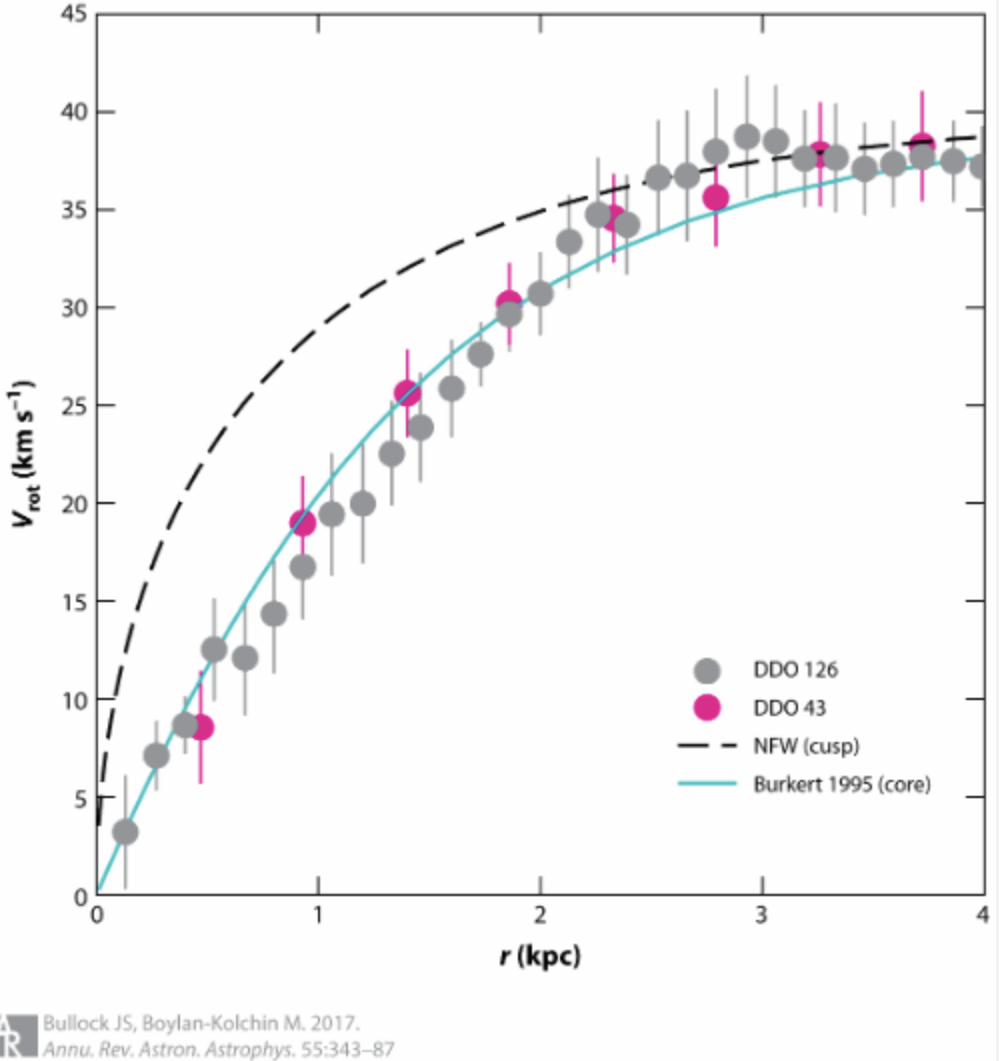
\includegraphics[width=0.48\textwidth]{Figures/cusp-coreVprof.png}
%  \end{center}
  \caption{Example of cusp-core problem from \cite{Bullock2017}. Dashed line is NFW expectation and points are two example galaxies. Galaxies are better fit with a constant-density core.}
  \label{cusp-core}
\end{wrapfigure}